%standard NAACL boilerplate header
\documentclass[11pt]{article}
\usepackage{naaclhlt2009}
\usepackage{times}
\usepackage{latexsym}
\setlength\titlebox{6.5cm}    % Expanding the titlebox

\usepackage{amsmath}				% want AMS fonts
\usepackage{amssymb}                            % use AMS symbols
\usepackage{graphicx}
\usepackage{rotating}
\usepackage{multirow}
%end NAACL boilerplate header
\usepackage{algorithm}
\usepackage[noend]{algorithmic}
\renewcommand{\algorithmiccomment}[1]{ // #1}

\newcommand{\cut}[1]{}
\newcommand{\commentw}[1]{{\bf WS: #1}}
\newcommand{\piecewise}[1]{\left\{\begin{array}{ll}#1\end{array}\right.}
\newcommand{\one}[1]{1\!\!1\left(#1\right)}
\newcommand{\R}{\mathbb{R}}                     % Reals.
\newcommand{\dotp}{\bullet}
\newcommand{\set}[1]{\{#1\}}			% Set (as in \set{1,2,3})
\newcommand{\setof}[2]{\{\,{#1}:{#2}\,\}}	% Set (as in \setof{x}{x > 0})
\newcommand{\alg}[1]{\textsc{#1}}

\title{Bounding and Comparing Methods for Correlation Clustering
  Beyond ILP}

\author{Micha Elsner and Warren Schudy\\
Department of Computer Science\\
Brown University \\
Providence, RI 02912 \\
  \{{\tt melsner,ws}\}{\tt @cs.brown.edu }}

\date{}

\begin{document}
\maketitle
\begin{abstract}
We evaluate several heuristic solvers for correlation clustering, the
NP-hard problem of partitioning a dataset given pairwise affinities
between all points. We experiment on two practical tasks, document
clustering and chat disentanglement, to which ILP does not scale. On
these datasets, we show that the clustering objective often, but not
always, correlates with external metrics, and that local search always
improves over greedy solutions. We use semi-definite programming (SDP)
to provide a tighter bound, showing that simple algorithms are already
close to optimality.
\end{abstract}

\section{Introduction}

Correlation clustering is a powerful technique for discovering
structure in data. It operates on the pairwise relationships between
datapoints, partitioning the graph to minimize the number of unrelated
pairs that are clustered together, plus the number of related pairs
that are separated. Unfortunately, this minimization problem is
NP-hard \cite{Ailon08}. Practical work has adopted one of three strategies for
solving it. For a few specific tasks, one can restrict the problem so
that it is efficiently solvable. In most cases, however, this is
impossible. Integer linear programming (ILP) can be used to solve the
general problem optimally, but only when the number of data points is
small. Beyond a few hundred points, the only available solutions are
heuristic or approximate.

In this paper, we evaluate a variety of solutions for correlation
clustering on two realistic NLP tasks, text topic clustering and chat
disentanglement, where typical datasets are too large for ILP to find
a solution. We show, as in previous work on consensus clustering
\cite{Goder08}, that local search can improve the solutions found
by commonly-used methods. We investigate the relationship between
the clustering objective and external evaluation metrics such as
F-score and one-to-one overlap, showing that optimizing the objective
is usually a reasonable aim, but that other measurements like number
of clusters found should sometimes be used to reject pathological
solutions.  We prove that the best heuristics are quite close to
optimal, using the first implementation of the semi-definite
programming (SDP) relaxation to provide tighter bounds.

The specific algorithms we investigate are, of course, only a subset
of the large number of possible solutions, or even of those proposed
in the literature. We chose to test a few common, efficient algorithms
that are easily implemented. Our use of a good bounding strategy means
that we do not need to perform an exhaustive comparison; we will show
that, though the methods we describe are not perfect, the remaining
improvements possible with any algorithm are relatively small.

\section{Previous Work}

Correlation clustering was first introduced by \newcite{BenDor99} to cluster gene expression patterns.  The correlation
clustering approach has several strengths. It does not require users
to specify a parametric form for the clusters, nor to pick the number
of clusters. Unlike fully unsupervised clustering methods, it can use
training data to optimize the pairwise classifier, but unlike
classification, it does not require samples from the specific clusters
found in the test data. For instance, it can use messages about
cars to learn a similarity function that can then be applied to
messages about atheism.

Correlation clustering is a standard method for coreference
resolution. It was introduced to the area by \newcite{Soon01}, who
describe the first-link heuristic method for solving
it. \newcite{Ng02} extend this work with better features, and develop
the best-link heuristic, which finds better
solutions. \newcite{McCallum05} explicitly describe the problem as
correlation clustering and use an approximate technique
\cite{Bansal04} to enforce transitivity. Recently \newcite{Finkel08}
show that the optimal ILP solution outperforms the first and best-link
methods. \newcite{Cohen02} experiment with various heuristic
solutions for the cross-document coreference task of grouping
references to named entities.

Finally, correlation clustering has proven useful in several discourse
tasks. \newcite{Barzilay06} use it for content aggregation in a
generation system. In \newcite{Malioutov06}, it is used for topic
segmentation---since segments must be contiguous, the problem can be
solved in polynomial time. \newcite{Elsner08a} address the related
problem of disentanglement (which we explore in Section \ref{chat}),
doing inference with the voting greedy algorithm.

\newcite{Bertolacci07}, \newcite{Goder08} and \newcite{Gionis07}
conduct experiments on the closely related problem of \emph{consensus
  clustering}, often solved by reduction to correlation
clustering. The input to this problem is a set of clusterings; the
output is a ``median'' clustering which minimizes the sum of (Rand)
distance to the inputs. Although these papers investigate some of the
same algorithms we use, they use an unrealistic lower bound, and so
cannot convincingly evaluate absolute performance. \newcite{Gionis07}
give an external evaluation on some UCI datasets, but this is
somewhat unconvincing since their metric, the {\em impurity index},
which is essentially precision ignoring recall, gives a perfect score to
the all-singletons clustering. The other two papers are based on objective values, not external metrics.\footnote{\newcite{Bertolacci07} gave normalized mutual information for one algorithm and data set, but almost all of their results study objective value only.}

%{\bf explain some theoretical work} 
A variety of approximation algorithms for correlation clustering with
worst-case theoretical guarantees have been proposed:
\cite{Bansal04,Ailon08,Demaine06,Charikar05,Giotis06}. Researchers
including \cite{BenDor99,Joachims05,Mathieu08a} study correlation
clustering theoretically when the input is generated by randomly
perturbing an unknown ground truth clustering. %As discussed later, we
%implement some of these algorithms.

\section{Algorithms}

We begin with some notation and a formal definition of the
problem. Our input is a complete, undirected graph $G$ with $n$ nodes;
each edge in the graph has a probability $p_{ij}$ reflecting our
belief as to whether nodes $i$ and $j$ come from the same cluster. Our
goal is to find a clustering, defined as a new graph $G'$ with edges
$x_{ij} \in \{0,1\}$, where if $x_{ij} = 1$, nodes $i$ and $j$ are
assigned to the same cluster. To make this consistent, the edges must
define an equivalence relationship: $x_{ii} = 1$ and $x_{ij} = x_{jk}
= 1$ implies $x_{ij} = x_{ik}$.

Our objective is to find a clustering as consistent as possible with
our beliefs---edges with high probability should not cross cluster
boundaries, and edges with low probability should. We define $w^+_{ij}$ as
the cost of cutting an edge whose probability is $p_{ij}$ and
$w^-_{ij}$ as the cost of keeping it. Mathematically, this objective
can be written \cite{Ailon08,Finkel08} as:
\begin{equation}
\min \sum_{ij:i<j} x_{ij}w^-_{ij} + (1 - x_{ij})w^+_{ij}.
\end{equation}
There are two plausible definitions for the costs $w^+$ and $w^-$,
both of which have gained some support in the literature. We can take
$w^+_{ij} = p_{ij}$ and $w^-_{ij} = 1 - p_{ij}$ ({\em additive}
weights) as in \cite{Ailon08} and others, or $w^+_{ij} = \log(p_{ij}),
w^-_{ij} = \log(1 - p_{ij})$ ({\em logarithmic} weights) as in
\cite{Finkel08}. The logarithmic scheme has a tenuous mathematical justification, since it selects a maximum-likelihood
clustering under the assumption that the $p_{ij}$ are independent and
identically distributed given the status of the edge $ij$ in the true
clustering. If we obtain the $p_{ij}$ using a classifier, however,
this assumption is obviously untrue---some nodes will be easy to link,
while others will be hard---so we evaluate the different weighting
schemes empirically.

%% \subsection{Linear Programming}

%% A clustering can be specified by indicator variables $x_{ij}$ for all distinct objects $i$ and $j$, where $x_{ij}$ has value 1 (true) if $i$ and $j$ are in the same cluster and 0 (false) otherwise. Let $x_{ij}$ and $x_{ji}$ denote the same variable.
%% % Equivalence relations are transitive, i.e. for all distinct $i,j,k$ if $x_{ij}$ and $x_{jk}$ then $x_{ik}$.
%% It is easy to see that indicator variables $x_{ij}$ correspond to a clustering if and only if they satisfy the \emph{transitivity} constraint $x_{ij} + x_{jk} - x_{ik} \leq 1$  for all distinct $i,j,k$. These constraints can also be written in a \emph{triangle inequality} form as $(1 - x_{ik}) \leq (1-x_{ij}) + (1-x_{jk})$. Correlation clustering is therefore equivalent to the following integer linear program:
%% \begin{eqnarray*}
%% & \min_{x} \sum_{i,j:i<j} x_{ij}w^-_{ij} + (1 - x_{ij})w^+_{ij}. \\
%% & \hbox{s.t.~}\left\{
%% \begin{array}{ll} 
%% x_{ij} + x_{jk} - x_{ik} \leq 1 & \forall \textrm{ distinct} i,j,k \\
%% x_{uv} \in \{0,1\}  &\forall \textrm{ distinct} u,v\\
%% \end{array}\right.
%% \end{eqnarray*}

%% Relaxing the constraint $x_{ij} \in \{0,1\}$ to $0 \leq x_{ij} \leq 1$ yields the standard LP relaxation of correlation clustering (e.g. \newcite{Ailon08}):
%% \begin{eqnarray*}
%% & \min_{x} \sum_{i,j:i<j} x_{ij}w^-_{ij} + (1 - x_{ij})w^+_{ij}. \\
%% & \hbox{s.t.~}\left\{
%% \begin{array}{ll} 0\leq x_{ij} \leq 1 &\forall \textrm{ distinct} i,j\\
%%  x_{ij} + x_{jk} - x_{ik} \leq 1 & \forall \textrm{ distinct} i,j,k
%% \end{array}\right.
%% \end{eqnarray*}

%%  For instances with sufficiently small clusters and high noise this is often LP optimal. \commentw{This observation is from playing with synthetic data. Move it to that section perhaps?}

\subsection{Greedy Methods}

We use four greedy methods drawn from the literature; they are both
fast and easy to implement.  All of them make decisions based on the
\emph{net weight} $w^{\pm}_{ij} = w^+_{ij} - w^{-}_{ij}$.

These algorithms step through the nodes of the graph according to a
permutation $\pi$. We try 100 random permutations for each algorithm
and report the run which attains the best objective value (typically
this is slightly better than the average run; we discuss this more in
the experimental sections). To simplify the pseudocode we label the
vertices $1,2,\ldots n$ in the order specified by $\pi$. After this
relabeling $\pi(i) = i$ so $\pi$ need not appear explicitly in the
algorithms.

Three of the algorithms are given in Figure~\ref{alg:bfv}. All three
algorithms start with the empty clustering and add the vertices one by
one. The \textsc{Best} algorithm adds each vertex $i$ to the
cluster with the strongest $w^\pm$ connecting to $i$, or to a new
singleton if none of the $w^\pm$ are positive. The \textsc{First}
algorithm adds each vertex $i$ to the cluster containing
the most recently considered vertex $j$ with $w^\pm_{ij} > 0$. The
\textsc{Vote} algorithm adds each vertex to the cluster that minimizes
the correlation clustering objective, i.e.\ to the cluster maximizing
the total net weight or to a singleton if no total is positive.

\newcite{Ailon08} introduced the \textsc{Pivot} algorithm, given in
Figure~\ref{alg:pivot}, and proved that it is a 5-approximation if
$w^+_{ij} + w^-_{ij} = 1$ for all $i,j$ and $\pi$ is chosen
randomly. Unlike \textsc{Best}, \textsc{Vote} and \textsc{First}, which build clusters vertex by
vertex, the \textsc{Pivot} algorithm creates each new cluster in its final
form. This algorithm repeatedly takes an unclustered pivot vertex and
creates a new cluster containing that vertex and all unclustered
neighbors with positive weight.

%%%%%%%%%%%%%%%%%%%%%%%%%%%%%%%%%%%%%%%%%%%%%%%%%%%%%%%%%%%%%%%%%%
\begin{figure}[bt]%%%%%%%%%%%%%%%
\begin{algorithmic}
%\STATE Relabel the vertices so that $\pi(i) = i$
\STATE $k \gets 0$ \COMMENT{number of clusters created so far}
\FOR{$i=1\ldots n$}
	\FOR{$c=1\ldots k$}
		\IF{\alg{Best}}
			\STATE $Quality_c \gets \max_{j \in C[c]} w^{\pm}_{ij}$
		\ELSIF{\alg{First}}
			\STATE $Quality_c \gets \max_{j \in C[c] : w^{\pm}_{ij} > 0} j$
		\ELSIF{\alg{Vote}}
			\STATE $Quality_c \gets \sum_{j \in C[c]} w^{\pm}_{ij}$
		\ENDIF
	\ENDFOR
	\STATE $c^* \gets \arg \max_{1 \leq c \leq k} Quality_c$
	\IF{$Quality_{c^*} > 0$}
		\STATE $C[c^*] \gets C[c^*] \cup \{i\}$
	\ELSE
		\STATE $C[k$++$] \gets \{i\}$ \COMMENT{form a new cluster}
	\ENDIF
\ENDFOR
\end{algorithmic}
\caption{\textsc{Best}/\textsc{First}/\textsc{Vote} algorithms}
\label{alg:bfv}
\end{figure}
%%%%%%%%%%%%%%%%%%%%%%%%%%%%%%%%%%%%%%%%%%%%%%%%%%%%%%%%%%%%%%%%%%

%%%%%%%%%%%%%%%%%%%%%%%%%%%%%%%%%%%%%%%%%%%%%%%%%%%%%%%%%%%%%%%%%%
\begin{figure}[bt]%%%%%%%%%%%%%%%
\begin{algorithmic}
%\STATE Relabel the vertices so that $\pi(i) = i$
\STATE $k \gets 0$ \COMMENT{number of clusters created so far}
\FOR{$i=1\ldots n$}
	\STATE $P \gets \bigcup_{1 \leq c \leq k} C[c]$ \COMMENT{Vertices already placed}
	\IF{$i \not \in P$}
		\STATE $C[k\textrm{++}] \gets \set{i} \cup \setof{i < j \leq
          n}{j \not\in P \textrm{ and } w^{\pm}_{ij} > 0}$
	\ENDIF
\ENDFOR
\end{algorithmic}
\caption{\textsc{Pivot} algorithm by \newcite{Ailon08}}
\label{alg:pivot}
\end{figure}
%%%%%%%%%%%%%%%%%%%%%%%%%%%%%%%%%%%%%%%%%%%%%%%%%%%%%%%%%%%%%%%%%%

\subsection{Local Search}

We use the straightforward local search previously used by
\newcite{Gionis07} and \newcite{Goder08}. The allowed \emph{one
  element moves} consist of removing one vertex from a cluster and
either moving it to another cluster or to a new singleton cluster. The
best one element move (\textsc{BOEM}) algorithm repeatedly makes the most
profitable best one element move until a local optimum is
reached. {\em Simulated Annealing} (\textsc{SA}) makes a random single-element
move, with probability related to the difference in objective it
causes and the current temperature. Our annealing schedule is
exponential and designed to attempt $2000n$ moves for $n$ nodes. We
initialize the local search either with all nodes clustered together,
or at the clustering produced by one of our greedy algorithms (in our
tables, the latter is written, eg. \textsc{Pivot}/\textsc{BOEM}, if the greedy algorithm
is \textsc{Pivot}).

\section{Bounding with SDP}\label{sec:sdp}

Although comparing different algorithms to one another gives a good
picture of relative performance, it is natural to wonder how well they
do in an absolute sense---how they compare to the optimal
solution. For very small instances, we can actually find the optimum
using ILP, but since this does not scale beyond a few hundred points
(see Section \ref{synthetic}), for realistic instances we must instead
bound the optimal value. Bounds are usually obtained by solving a {\em
  relaxation} of the original problem: a simpler problem with the same
objective but fewer constraints.

The bound used in previous work \cite{Goder08,Gionis07,Bertolacci07},
which we call the {\em trivial bound}, is obtained by ignoring the
transitivity constraints entirely. To optimize, we link ($x_{ij} = 1$)
all the pairs where $w^+_{ij}$ is larger than $w^-_{ij}$; since this
solution is quite far from being a clustering, the bound tends not to
be very tight.

To get a better idea of how good a real clustering can be, we use
a semi-definite programming (SDP) relaxation to provide a better
bound. Here we motivate and define this relaxation.

One can picture a clustering geometrically by associating cluster $c$
with the standard basis vector $e_c =
(\underbrace{0,0,\ldots,0,}_{c-1}1,\underbrace{0,\ldots,0}_{n-c}) \in
\R^n$. If object $i$ is in cluster $c$ then it is natural to associate
$i$ with the vector $r_i=e_c$. This gives a nice geometric picture of
a clustering, with objects $i$ and $j$ in the same cluster if and only
if $r_i = r_j$. Note that the dot product $r_i \dotp r_j$ is 1 if $i$
and $j$ are in the same cluster and 0 otherwise. These ideas yield a
simple reformulation of the correlation clustering problem:
\begin{eqnarray*}
& \min_{r} \sum_{i,j:i<j} (r_i \dotp r_j)w^-_{ij} + (1 - r_j \dotp r_j) w^+_{ij} \\
& \hbox{s.t.~}
%\left\{
%\begin{array}{ll}
\forall i~~\exists c : r_i=e_c
%\end{array}\right.
\end{eqnarray*}
%Note the $r_i$ are not necessarily distinct and need not form a basis themselves.

To get an efficiently computable lower-bound we relax the constraints
that the $r_i$s are standard basis vectors, replacing them with two
sets of constraints: $r_i \dotp r_i = 1$ for all $i$ and $r_i \dotp
r_j \geq 0$ for all $i,j$.

%%  This yields the standard vector program relaxation of correlation clustering:
%% \begin{eqnarray*}
%% & \min_{r} \sum_{i,j:i<j} (r_i \dotp r_j)w^-_{ij} + (1 - r_j \dotp r_j) w^+_{ij} \\
%% & \hbox{s.t.~}
%% \left\{
%% \begin{array}{ll}
%% r_i \dotp r_i = 1 & \forall i \\
%% r_i \dotp r_j \geq 0 & \forall i\neq j
%% \end{array}\right.
%% \end{eqnarray*}
%% %The above vector program only depends on the vectors $r_i$ through the dot products 

Since the $r_i$ only appear as dot products, we can rewrite in terms
of $x_{ij} = r_i \dotp r_j$. However, we must now constrain the
$x_{ij}$ to be the dot products of some set of vectors in $\R^n$. This
is true if and only if the symmetric matrix $X=\{x_{ij}\}_{ij}$ is
\emph{positive semi-definite}. We now have the standard semi-definite
programming (SDP) relaxation of correlation clustering
(e.g. \cite{Charikar05,Mathieu08a}):
\begin{eqnarray*}
& \min_{x} \sum_{i,j:i<j} x_{ij}w^-_{ij} + (1 - x_{ij})w^+_{ij} \\
& \hbox{s.t.~}\left\{
\begin{array}{ll} 
x_{ii} = 1 & \forall i \\
x_{ij} \geq 0 & \forall i,j \\
X=\{x_{ij}\}_{ij} \textrm{ PSD} &
\end{array}\right.
.\end{eqnarray*}

This SDP has been studied theoretically by a number of authors; we
mention just two here. \newcite{Charikar05} give an approximation
algorithm based on rounding the SDP which is a 0.7664 approximation
for the problem of maximizing agreements. \newcite{Mathieu08a} show
that if the input is generated by corrupting the edges of a ground
truth clustering $B$ independently, then the SDP relaxation value is
within an additive $O(n \sqrt n)$ of the optimum clustering. They
further show that using the \alg{Pivot} algorithm to round the SDP yields a
clustering with value at most $O(n \sqrt n)$ more than optimal.
% optimum is very close to the ground truth clustering, i.e.\ the Rand index $\sum_{ij} |B_{ij} - x^*_{ij}| = \theta(n \sqrt n)$.

\section{Experiments}

\subsection{Scalability}
\label{synthetic}

%% {\bf possibly we want some synthetic data with timing curves to show
%%   that ILP really doesn't scale}

%% \commentw{Even better, we can show that the LP doesn't scale, never mind the ILP part!}

%% \commentw{I just ran a quick test on sunlab machines and a 200 instance to double-check that laziness helps; lazplp took 70 seconds whereas non-lazy took 870 seconds before running out of memory.}

Using synthetic data, we investigate the scalability of the linear
programming solver and SDP bound. To find optimal solutions, we pass
the complete ILP\footnote{Consisting of the objective plus constraints
  $0 \le x_{ij} \le 1$ and triangle inequality \cite{Ailon08}.} to
CPLEX. This is reasonable for 100 points and solvable for 200; beyond
this point it cannot be solved due to memory exhaustion. As noted
below, despite our inability to compute the LP bound on large
instances, we can sometimes prove that they must be worse than SDP
bounds, so we do not investigate LP-solving techniques further.

%% We use synthetic data to investigate the scalability of the linear
%% programming solver and SDP bound. We sample a random dataset for every
%% size between 100 and 1000; the datapoints are drawn from spherical
%% Gaussians, and the pairwise classifications are logistic regression on
%% coordinate differences.

The SDP has fewer constraints than the ILP ($O(n^2)$ vs $O(n^3)$), but
this is still more than many SDP solvers can handle. For our
experiments we used one of the few SDP solvers that can handle such a
large number of constraints: Christoph Helmberg's ConicBundle library \cite{Helmberg09,Helmberg00}. This solver can handle several
thousand datapoints. It produces loose lower-bounds (off by a few
percent) quickly but converges to optimality quite slowly; we err on
the side of inefficiency by running for up to 60 hours. Of course, the
SDP solver is only necessary to bound algorithm performance; our
solvers themselves scale much better.


%% Interestingly, CPLEX cannot
%% even solve the LP relaxation much beyond this point, although it is
%% theoretically solvable in polynomial time. Our experience matches
%% \newcite{Bertolacci07}, who report they could solve the LP for 256
%% vertices but not 512.

%% In the $n^2/2$ dimensional search space only $n^2/2$ constraints are
%% sufficient to specify a vertex. This is far less than the roughly
%% $n^3/2$ total triangle inequality constraints, which suggests adding
%% the constraints lazily.  Our lazy LP solver begins by solving the LP
%% with no triangle constraints. We then pick $n^2 / 2$ constraints at
%% random from the set of violated constraints and add those to the
%% LP. We repeatedly solve the LP and add batches of $n^2 /2$ new
%% constraints until no constraints are violated. The lazy addition of
%% constraints dramatically improves scalability, but even so we could
%% not solve the LP above xxxx {\bf still checking} objects.



\subsection{Twenty Newsgroups}

In this section, we test our approach on a typical benchmark
clustering dataset, 20 Newsgroups, which contains posts from a variety
of Usenet newsgroups such as \texttt{rec.motorcycles} and
\texttt{alt.atheism}. Since our bounding technique does not scale to
the full dataset, we restrict our attention to a subsample of 100
messages\footnote{Available as \texttt{mini\_newsgroups.tar.gz} from
  the UCI machine learning repository.}  from each newsgroup for a
total of 2000---still a realistically large-scale problem. Our goal is
to cluster messages by their newsgroup of origin. We conduct
experiments by holding out four newsgroups as a training set, learning
a pairwise classifier, and applying it to the remaining 16 newsgroups
to form our affinity matrix.\footnote{The experiments below are
  averaged over four disjoint training sets.}

Our pairwise classifier uses three types of features previously found
useful in document clustering. First, we bucket all words\footnote{We
  omit the message header, except the subject line, and also discard
  word types with fewer than 3 occurrences.} by their log document
frequency (for an overview of TF-IDF see \cite{Joachims97a}). For a
pair of messages, we create a feature for each bucket whose value is
the proportion of shared words in that bucket. Secondly, we run LSA
\cite{Deerwester90} on the TF-IDF matrix for the dataset, and use the
cosine distance between each message pair as a feature. Finally, we
use the same type of shared words features for terms in message
subjects. We make a training instance for each pair of documents in
the training set and learn via logistic regression.

%% P: 27.05 R: 36.36 F: 31.02 Acc: 90 (1151116/1279200) (28799/79200)
%% P: 23.26 R: 39.95 F: 29.40 Acc: 88 (1127260/1279200) (31643/79200)
%% P: 23.78 R: 34.66 F: 28.21 Acc: 89 (1139477/1279200) (27450/79200)
%% P: 21.96 R: 41.94 F: 28.83 Acc: 87 (1115192/1279200) (33220/79200)

The classifier has an average F-score of 29\% and an accuracy of
88\%---not particularly good. We should emphasize that the clustering
task for 20 newsgroups is much harder than the more common
classification task---since our training set is entirely disjoint with
the testing set, we can only learn weights on feature categories, not
term weights. Our aim is to create realistic-looking data on which to
test our clustering methods, not to motivate correlation clustering as
a solution to this specific problem. In fact, \newcite{Zhong03} report
better results using generative models.

We evaluate our clusterings using three different metrics (see
\newcite{Meila07} for an overview of clustering metrics). The {\em
  Rand} measure counts the number of pairs of points for which the
proposed clustering agrees with ground truth. This is the metric which
is mathematically closest to the objective. However, since most points
are in different clusters, any solution with small clusters tends to
get a high score. Therefore we also report the more sensitive {\em
  F-score} with respect to the minority (``same cluster'') class. We
also report the {\em one-to-one} score, which measures accuracy over
single points. For this metric, we calculate a maximum-weight matching
between proposed clusters and ground-truth clusters, then report the
overlap between the two.

\begin{table}[bt!]
\begin{tabular}{l|c|c|c|c}
\multicolumn{5}{c}{Logarithmic Weights}
\\ \hline
 & Obj & Rand & F & 1-1
\\ \hline
SDP bound & 51.1\% & - & - & - 
\\ \hline
\alg{Vote}/\alg{BOEM} & 55.8\% & 93.80 & 33 & 41
\\ 
SA & 56.3\% & 93.56 & 31 & 36
\\ 
\alg{Pivot}/\alg{BOEM} & 56.6\% & 93.63 & 32 & 39
\\ 
\alg{Best}/\alg{BOEM} & 57.6\% & 93.57 & 31 & 38
\\ 
\alg{First}/\alg{BOEM} & 57.9\% & 93.65 & 30 & 36
\\ 
\alg{Vote} & 59.0\% & 93.41 & 29 & 35
\\ 
\alg{BOEM} & 60.1\% & 93.51 & 30 & 35
\\ 
\alg{Pivot} & 100\% & 90.85 & 17 & 27
\\ 
\alg{Best} & 138\% & 87.11 & 20 & 29
\\ 
\alg{First} & 619\% & 40.97 & 11 & 8
\\ 
\multicolumn{5}{c}{}\\
\multicolumn{5}{c}{Additive Weights}
\\ \hline
 & Obj & Rand & F & 1-1
\\ \hline
SDP bound & 59.0\% & - & - & -
\\ \hline
SA & 63.5\% & 93.75 & 32 & 39
\\ 
\alg{Vote}/\alg{BOEM} & 63.5\% & 93.75 & 32 & 39
\\ 
\alg{Pivot}/\alg{BOEM} & 63.7\% & 93.70 & 32 & 39
\\ 
\alg{Best}/\alg{BOEM} & 63.8\% & 93.73 & 31 & 39
\\ 
\alg{First}/\alg{BOEM} & 63.9\% & 93.58 & 31 & 37
\\ 
\alg{BOEM} & 64.6\% & 93.65 & 31 & 37
\\ 
\alg{Vote} & 67.3\% & 93.35 & 28 & 34
\\ 
\alg{Pivot} & 109\% & 90.63 & 17 & 26
\\ 
\alg{Best} & 165\% & 87.06 & 20 & 29
\\ 
\alg{First} & 761\% & 40.46 & 11 & 8
\\ 
\end{tabular}
\caption{Score of the solution with best objective for
  each solver, averaged over newsgroups training sets, sorted by objective.}
\label{newsgroup-results}
\end{table}

When presenting objective values, we locate them within the range
between the trivial lower bound discussed in Section \ref{sec:sdp} and the
objective value of the singletons clustering ($x_{ij} = 0, i \ne
j$). On this scale, lower is better; 0\% corresponds to the trivial
bound and 100\% corresponds to the singletons clustering. It is
possible to find values greater than 100\%, since some particularly
bad clusterings have objectives worse than the singletons
clustering. Plainly, however, real clusterings will not have values as
low as 0\%, since the trivial bound is so unrealistic.

Our results are shown in Table \ref{newsgroup-results}. The best
results are obtained using logarithmic weights with \alg{Vote}
followed by \alg{BOEM}; reasonable results are also found using
additive weights, and annealing, \alg{Vote} or \alg{Pivot} followed by
\alg{BOEM}. On its own, the best greedy scheme is \alg{Vote}, but all
of them are substantially improved by \alg{BOEM}. First-link is by far
the worst. Our use of the SDP lower bound rather than the trivial
lower-bound of 0\% reduces the gap between the best clustering and the
lower bound by over a factor of ten. It is easy to show that the LP
relaxation can obtain a bound of at most 50\%\footnote{The solution
  $x_{ij} = \frac{1}{2} \one{w^-_{ij} > w^+_{ij}}$ for $i < j$ is
  feasible in the LP.}---the SDP beats the LP in both runtime and
quality!

We analyze the correlation between objective values and metric values,
averaging Kendall's tau\footnote{The standard Pearson correlation
  coefficient is less robust to outliers, which causes problems for
  this data.} over the four datasets (Table \ref{correlations}). Over
the entire dataset, correlations are generally good (large and
negative), showing that optimizing the objective is indeed a useful
way to find good results. We also examine correlations for the
solutions with objective values within the top 10\%. Here the
correlation is much poorer; selecting the solution with the best
objective value will not necessarily optimize the metric, although the
correspondence is slightly better for the log-weights scheme. The
correlations do exist, however, and so the solution with the best
objective value is typically slightly better than the median.

In Figure \ref{box}, we show the distribution of one-to-one scores
obtained (for one specific dataset) by the best solvers. From this
diagram, it is clear that log-weights and \alg{Vote}/\alg{BOEM} usually obtain the
best scores for this metric, since the median is higher than other
solvers' upper quartile scores. All solvers have quite high variance,
with a range of about 2\% between quartiles and 4\% overall. We omit
the F-score plot, which is similar, for space reasons.

\begin{figure}[bt!]
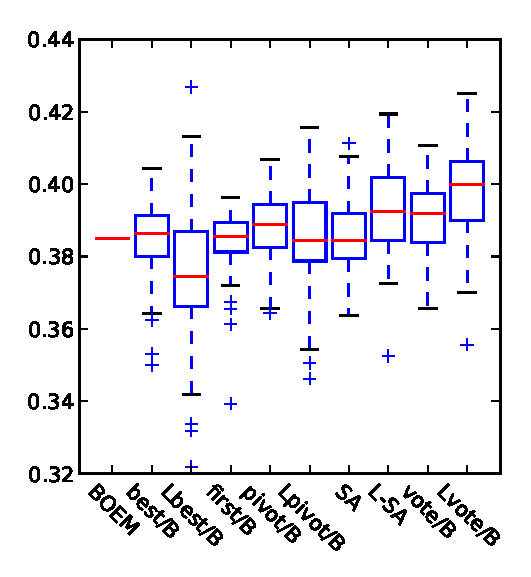
\includegraphics{box-tiny-3.eps}
\caption{Box-and-whisker diagram (outliers as $+$) for one-to-one
  scores obtained by the best few solvers on a particular newsgroup
  dataset. L means using log weights. B means improved with \alg{BOEM}.}
\label{box}
\end{figure}

\begin{table}
\begin{tabular}{l|ccc}
& Rand & F & 1-1\\
\hline
Log-wt & -.60 & -.73 & -.71\\
Top 10 \% & -.14 & -.22 & -.24\\
\hline
Add-wt & -.60 & -.67 & -.65\\
Top 10 \% & -.13 & -.15 & -.14
\end{tabular}
\caption{Kendall's tau correlation between objective and metric
  values, averaged over newsgroup datasets, for all solutions and top
  10\% of solutions.}
\label{correlations}
\end{table}

%% spearman's r -- pretty similar to tau scores really
%% 121 mean -0.880297657432 10 -0.353300330033
%% f mean -0.907351396358 10 -0.3150060006
%% rand mean -0.744563534519 10 -0.206011851185
%% add
%% 121 mean -0.830303170632 10 -0.206130363036
%% f mean -0.862035729989 10 -0.232652265227
%% rand mean -0.742914632523 10 -0.183696369637

%% \begin{table}
%% \begin{tabular}{|c|c|}
%%  & clusters
%% \\ \hline
%% log best & 12
%% \\ \hline
%% log first & 12
%% \\ \hline
%% log vote boem & 106
%% \\ \hline
%% log first boem & 99
%% \\ \hline
%% log boem & 99
%% \\ \hline
%% log pivot & 61
%% \\ \hline
%% log vote & 98
%% \\ \hline
%% log pivot boem & 106
%% \\ \hline
%% log sa boem & 132
%% \\ \hline
%% log best boem & 101
%% \\ \hline
%%  & clusters
%% \\ \hline
%% vote boem & 108
%% \\ \hline
%% sa boem & 114
%% \\ \hline
%% first boem & 107
%% \\ \hline
%% pivot boem & 109
%% \\ \hline
%% best & 12
%% \\ \hline
%% first & 12
%% \\ \hline
%% best boem & 108
%% \\ \hline
%% vote & 103
%% \\ \hline
%% boem & 107
%% \\ \hline
%% pivot & 61
%% \\ \hline
%% \end{tabular}
%% \caption{clusters fnd}
%% \end{table}


\subsection{Chat Disentanglement}
\label{chat}

In the disentanglement task, we examine data from a shared discussion
group where many conversations are occurring simultaneously. The task
is to partition the utterances into a set of conversations. This task
differs from newsgroup clustering in that data points (utterances)
have an inherent linear order. Ordering is typical in discourse tasks
including topic segmentation and coreference resolution.

We use the annotated dataset and pairwise classifier made available by
\newcite{Elsner08a};\footnote{Downloaded from
  \texttt{cs.brown.edu/$\sim$melsner}} this study represents a
competitive baseline, although more recently \newcite{Wang09} have
improved it. Since this classifier is ineffective at linking
utterances more than 129 seconds apart, we treat all decisions for
such utterances as abstentions, $p=.5$. For utterance pairs on which
it does make a decision, the classifier has a reported accuracy of
75\% with an F-score of 71\%.

As in previous work, we run experiments on the 800-utterance test set
and average metrics over 6 test annotations. We evaluate using the
three metrics reported by previous work. Two node-counting metrics
measure global accuracy: {\em one-to-one match} as explained above,
and {\em Shen's F} \cite{Shen06}:
%\begin{equation*}
$
F = \sum_i \frac{n_i}{n}\max_j(F(i,j))
$.
%\end{equation*}
Here $i$ is a gold conversation with size $n_i$ and $j$ is a proposed
conversation with size $n_j$, sharing $n_{ij}$ utterances; $F(i,j)$ is
the harmonic mean of precision ($\frac{n_{ij}}{n_j}$) and recall
($\frac{n_{ij}}{n_i}$). A third metric, the {\em local agreement},
counts edgewise agreement for pairs of nearby utterances, where nearby
means ``within three utterances.''

In this dataset, the SDP is a more moderate improvement over the
trivial lower bound, reducing the gap between the best clustering and
best lower bound by a factor of about 3 (Table \ref{chat-test}).

Optimization of the objective does not correspond to improvements in
the global metrics (Table \ref{chat-test}); for instance, the best
objectives are attained with \alg{First}/\alg{BOEM}, but
\alg{Vote}/\alg{BOEM} yields better one-to-one and F
scores. Correlation between the objective and these global metrics is
extremely weak \cut{or slightly anti-correlated} (Table
\ref{test-chat-correlation}). The local metric is somewhat correlated.

Local search does improve metric results for each particular greedy
algorithm. For instance, when \alg{BOEM} is added to \alg{Vote} (with log
weights), one-to-one increases from 44\% to 46\%, local from 72\% to
73\% and F from 48\% to 50\%. This represents a moderate improvement
on the inference scheme described in \newcite{Elsner08a}. They use
voting with additive weights, but rather than performing multiple runs
over random permutations, they process utterances in the order they
occur. (We experimented with processing in order; the results are
unclear, but there is a slight trend toward worse performance, as in
this case.) Their results (also shown in the table) are 41\%
one-to-one, 73\% local and .44\% F-score.\footnote{The F-score metric
  is not used in \newcite{Elsner08a}; we compute it ourselves on the
  result produced by their software.} Our improvement on the global
metrics (12\% relative improvement in one-to-one, 13\% in F-score) is
modest, but was achieved with better inference on exactly the
same input.

Since the objective function fails to distinguish good solutions from
bad ones, we examine the types of solutions found by different methods
in the hope of explaining why some perform better than others. In this
setting, some methods (notably local search run on its own or from a
poor starting point) find far fewer clusters than others (Table
\ref{nclusters}; log weights not shown but similar to additive). Since
the classifier abstains for utterances more than 129 seconds apart,
the objective is unaffected if very distant utterances are linked on
the basis of little or no evidence; this is presumably how such large
clusters form. (This raises the question of whether abstentions
should be given weaker links with $p < .5$. We leave this for future
work.)  Algorithms which find reasonable numbers of clusters
(\alg{Vote}, \alg{Pivot}, \alg{Best} and local searches based on
these) all achieve good metric scores, although there is still no
reliable way to find the best solution among this set of methods.

\begin{table}[th!]
\begin{tabular}{l|cccc}
\multicolumn{5}{c}{Log Weights}\\
\hline
 & Obj & 1-1 & $Loc_3$ & Shen F
\\ \hline
SDP bound & 13.0\% & - & - & -
\\ \hline
\alg{First}/\alg{BOEM} & 19.3\% & 41 & {\bf 74} & 44
\\ 
\alg{Vote}/\alg{BOEM} & 20.0\% & {\bf 46} & {\bf 73} & {\bf 50}
\\ 
SA & 20.3\% & 42 & {\bf 73} & 45
\\ 
\alg{Best}/\alg{BOEM} & 21.3\% & 43 & {\bf 73} & 47
\\ 
\alg{BOEM} & 21.5\% & 22 & 72 & 21
\\ 
\alg{Pivot}/\alg{BOEM} & 22.0\% & {\bf 45} & 72 & {\bf 50}
\\ 
\alg{Vote} & 26.3\% & 44 & 72 & 48
\\ 
\alg{Best} & 37.1\% & 40 & 67 & 44
\\ 
\alg{Pivot} & 44.4\% & 39 & 66 & 44
\\ 
\alg{First} & 58.3\% & 39 & 62 & 41
\\ 




%% \\ \hline
%% sdp2l p b & -2.35e+05 & 0.39 & 0.73 & 0.42
%% \\ \hline
%% first boem & -2.34e+05 & 0.41 & 0.74 & 0.44
%% \\ \hline
%% vote boem & -2.34e+05 & 0.46 & 0.73 & 0.5
%% \\ \hline
%% sa boem & -2.34e+05 & 0.42 & 0.73 & 0.45
%% \\ \hline
%% best boem & -2.34e+05 & 0.43 & 0.73 & 0.47
%% \\ \hline
%% boem & -2.34e+05 & 0.22 & 0.72 & 0.21
%% \\ \hline
%% pivot boem & -2.34e+05 & 0.45 & 0.72 & 0.5
%% \\ \hline
%% vote & -2.33e+05 & 0.44 & 0.72 & 0.48
%% \\ \hline
%% best & -2.32e+05 & 0.40 & 0.67 & 0.44
%% \\ \hline
%% pivot & -2.31e+05 & 0.39 & 0.66 & 0.44
%% \\ \hline
%% first & -2.29e+05 & 0.39 & 0.62 & 0.41
%% \\ \hline
\multicolumn{5}{c}{}\\
\multicolumn{5}{c}{Additive Weights}
\\ \hline
 & Obj & 1-1 & $Loc_3$ & Shen F
\\ \hline
SDP bound & 16.2\% & - & - & -
\\ \hline
\alg{First}/\alg{BOEM} & 21.7\% & 40 & {\bf 73} & 44
\\ 
\alg{BOEM} & 22.3\% & 22 & {\bf 73} & 20
\\ 
\alg{Best}/\alg{BOEM} & 22.7\% & 44 & {\bf 74} & {\bf 49}
\\ 
\alg{Vote}/\alg{BOEM} & 23.3\% & {\bf 46} & {\bf 73} & {\bf 50}
\\ 
SA & 23.8\% & 41 & 72 & 46
\\ 
\alg{Pivot}/\alg{BOEM} & 24.8\% & {\bf 46} & 73 & {\bf 50}
\\ 
\alg{Vote} & 30.5\% & 44 & 71 & {\bf 49}
\\ 
{\em EC '08} & - & 41 & {\bf 73} & 44
\\
\alg{Best} & 42.1\% & 43 & 69 & 47
\\ 
\alg{Pivot} & 48.4\% & 38 & 67 & 44
\\ 
\alg{First} & 69.0\% & 40 & 59 & 41



%% \\ \hline
%% sdp2l p b & 1.57e+05 & 0.40 & 0.73 & 0.42
%% \\ \hline
%% first boem & 1.57e+05 & 0.40 & 0.73 & 0.44
%% \\ \hline
%% boem & 1.57e+05 & 0.22 & 0.73 & 0.2
%% \\ \hline
%% best boem & 1.57e+05 & 0.44 & 0.74 & 0.49
%% \\ \hline
%% vote boem & 1.57e+05 & 0.46 & 0.73 & 0.5
%% \\ \hline
%% sa boem & 1.57e+05 & 0.41 & 0.72 & 0.46
%% \\ \hline
%% pivot boem & 1.57e+05 & 0.46 & 0.73 & 0.5
%% \\ \hline
%% vote & 1.57e+05 & 0.44 & 0.71 & 0.49
%% \\ \hline
%% EC '08 & - & 0.41 & 0.73 & .44
%% \\ \hline
%% best & 1.58e+05 & 0.43 & 0.69 & 0.47
%% \\ \hline
%% pivot & 1.58e+05 & 0.39 & 0.67 & 0.44
%% \\ \hline
%% first & 1.59e+05 & 0.40 & 0.59 & 0.41
%% \\ \hline
\end{tabular}
\caption{Score of the solution with best objective found by
  each solver on the chat test dataset, averaged over 6 annotations,
  sorted by objective.}
\label{chat-test}
\end{table}

\begin{table}
\begin{tabular}{l|c|}
 & Num clusters
\\ \hline
{\em Max human annotator} & {\em 128}\\
\alg{Pivot} & 122\\
\alg{Vote} & 99\\
\alg{Pivot}/\alg{BOEM} & 89\\
\alg{Vote}/\alg{BOEM} & 86\\
{\em Mean human annotator} & {\em 81}\\
\alg{Best} & 70\\
\alg{First} & 70\\
{\em \newcite{Elsner08a}} & {\em 63}\\
\alg{Best}/\alg{BOEM} & 62\\
SA & 57\\
\alg{First}/\alg{BOEM} & 54\\
{\em Min human annotator} & {\em 50}\\
\alg{BOEM} & 7
\end{tabular}
\caption{Average number of clusters found (using additive weights) for
  chat test data.}
\label{nclusters}
\end{table}


%% \begin{table}
%% \begin{tabular}{|c|c|}
%% \hline
%%  & clusters
%% \\ \hline
%% log best & 69
%% \\ \hline
%% log first & 69
%% \\ \hline
%% log best boem & 62
%% \\ \hline
%% log vote boem & 85
%% \\ \hline
%% log first boem & 53
%% \\ \hline
%% log boem & 7
%% \\ \hline
%% log pivot & 123
%% \\ \hline
%% log vote & 97
%% \\ \hline
%% log pivot boem & 89
%% \\ \hline
%% log sdp2l pivot boem & 63
%% \\ \hline
%% log sa boem & 69
%% \\ \hline
%%  & clusters
%% \\ \hline
%% vote boem & 86
%% \\ \hline
%% sa boem & 57
%% \\ \hline
%% first boem & 54
%% \\ \hline
%% pivot boem & 89
%% \\ \hline
%% best & 70
%% \\ \hline
%% first & 70
%% \\ \hline
%% sdp2l pivot boem & 65
%% \\ \hline
%% best boem & 62
%% \\ \hline
%% vote & 99
%% \\ \hline
%% boem & 7
%% \\ \hline
%% pivot & 122
%% \\ \hline
%% \end{tabular}
%% \end{table}

\begin{table}[th!]
\begin{tabular}{l|ccc}
& 1-1 & $Loc_3$ & Shen F\\
\hline
Log-wt & -.40 & -.68 & -.35\\
Top 10 \% & .14 & -.15 & .15\\
\hline
Add-wt & -.31 & -.67 & -.25\\
Top 10 \% & -.07 & -.22 & .13\\
\end{tabular}
\caption{Kendall's tau correlation between objective and metric
  values for the chat test set, for all solutions and top
  10\% of solutions.}
\label{test-chat-correlation}
\end{table}

\section{Conclusions}

It is clear from these results that heuristic methods can provide good
correlation clustering solutions on datasets far too large for ILP to
scale. The particular solver chosen\footnote{Our C++ correlation
  clustering software and SDP bounding package are available for
  download from \texttt{cs.brown.edu/$\sim$melsner}.} has a
substantial impact on the quality of results obtained, in terms of
external metrics as well as objective value.

For general problems, our recommendation is to use log weights and run
\alg{Vote}/\alg{BOEM}. This algorithm is fast, achieves good objective values,
and yields good metric scores on our datasets. Although objective
values are usually only weakly correlated with metrics, our results
suggest that slightly better scores can be obtained by running the
algorithm many times and returning the solution with the best
objective. This may be worth trying even when the datapoints
are inherently ordered, as in chat.

Whatever algorithm is used to provide an initial solution, we advise
the use of local search as a post-process. \alg{BOEM} always improves both
objective and metric values over its starting point.

The objective value is not always sufficient to select a good solution
(as in the chat dataset). If possible, experimenters should check
statistics like the number of clusters found to make sure they conform
roughly to expectations. Algorithms that find far too many or too few
clusters, regardless of objective, are unlikely to be useful. This
type of problem can be especially dangerous if the pairwise classifier
abstains for many pairs of points.

SDP provides much tighter bounds than the trivial bound used in
previous work, although how much tighter varies with dataset (about 12
times smaller \cut{gap} for newsgroups, 3 times \cut{smaller gap} for
chat). This bound can be used to evaluate the absolute performance of
our solvers; the \alg{Vote}/\alg{BOEM} solver whose use we recommend
is within about 5\% of optimality. Some of this 5\% represents the
difference between the bound and optimality; the rest is the
difference between the optimum and the solution found. If the
bound were exactly optimal\cut{ the entire 5\% were achievable
  (\cut{that is,}the SDP bound \cut{value} was optimal \cut{were
    identical to optimum})}, we could expect a significant improvement
on our best results, but not a very large one---especially since
correlation between objective and metric values grows weaker for the
best solutions. While it might be useful to investigate more
sophisticated local searches in an attempt to close the gap, we do not
view this as a priority.

%% A more interesting direction for future work might be to adapt
%% algorithms, and the SDP bounding method, to other NLP problems
%% typically solved with ILP \cite{Roth04}. {\bf say more here?}

\section*{Acknowledgements}
 We thank Christoph Helmberg, Claire Mathieu and three reviewers.

%% Suppressed to preserve anonymity. Claire belongs on this list.
%% Christoph Helmberg for assistance with his ConicBundle solver.

\bibliographystyle{naaclhlt2009}
\bibliography{bllip}

\end{document}



%% \begin{table}
%% \begin{tabular}{|c|c|c|c|c|}
%% \multicolumn{5}{c}{Log Weights}\\

%% \hline
%%  & obj & 121 & loc3 & shenf
%% \\ \hline
%% sdp2l p b & -2.35e+05 & 0.39 & 0.73 & 0.42
%% \\ \hline
%% vote-id boem & -2.34e+05 & 0.409 & 0.73 & 0.44
%% \\ \hline
%% first boem & -2.34e+05 & 0.406 & 0.74 & 0.44
%% \\ \hline
%% $\Rightarrow$ vote-id & -2.34e+05 & 0.416 & 0.73 & 0.44
%% \\ \hline
%% vote boem & -2.34e+05 & 0.46 & 0.73 & 0.5
%% \\ \hline
%% sa boem & -2.34e+05 & 0.42 & 0.73 & 0.45
%% \\ \hline
%% best-id boem & -2.34e+05 & 0.355 & 0.74 & 0.36
%% \\ \hline
%% best boem & -2.34e+05 & 0.427 & 0.73 & 0.47
%% \\ \hline
%% boem & -2.34e+05 & 0.223 & 0.72 & 0.21
%% \\ \hline
%% pivot boem & -2.34e+05 & 0.448 & 0.72 & 0.5
%% \\ \hline
%% first-id boem & -2.34e+05 & 0.354 & 0.73 & 0.38
%% \\ \hline
%% vote & -2.33e+05 & 0.436 & 0.72 & 0.48
%% \\ \hline
%% pivot-id boem & -2.33e+05 & 0.445 & 0.71 & 0.5
%% \\ \hline
%% best & -2.32e+05 & 0.401 & 0.67 & 0.44
%% \\ \hline
%% sa & -2.32e+05 & 0.34 & 0.65 & 0.4
%% \\ \hline
%% best-id & -2.31e+05 & 0.376 & 0.67 & 0.37
%% \\ \hline
%% pivot & -2.31e+05 & 0.387 & 0.66 & 0.44
%% \\ \hline
%% pivot-id & -2.3e+05 & 0.354 & 0.67 & 0.42
%% \\ \hline
%% first & -2.29e+05 & 0.392 & 0.62 & 0.41
%% \\ \hline
%% first-id & -2.29e+05 & 0.369 & 0.57 & 0.36
%% \\ \hline

%% \multicolumn{5}{c}{Additive Weights {\bf separate table?}}\\
%%  & obj & 121 & loc3 & shenf
%% \\ \hline
%% sdp2l p b & 1.57e+05 & 0.396 & 0.73 & 0.42
%% \\ \hline
%% vote-id boem & 1.57e+05 & 0.407 & 0.73 & 0.44
%% \\ \hline
%% first boem & 1.57e+05 & 0.403 & 0.73 & 0.44
%% \\ \hline
%% best-id boem & 1.57e+05 & 0.347 & 0.74 & 0.36
%% \\ \hline
%% $\Rightarrow$ vote-id & 1.57e+05 & 0.414 & 0.73 & 0.44
%% \\ \hline
%% boem & 1.57e+05 & 0.216 & 0.73 & 0.2
%% \\ \hline
%% best boem & 1.57e+05 & 0.444 & 0.74 & 0.49
%% \\ \hline
%% vote boem & 1.57e+05 & 0.456 & 0.73 & 0.5
%% \\ \hline
%% first-id boem & 1.57e+05 & 0.352 & 0.73 & 0.37
%% \\ \hline
%% sa boem & 1.57e+05 & 0.406 & 0.72 & 0.46
%% \\ \hline
%% pivot boem & 1.57e+05 & 0.457 & 0.73 & 0.5
%% \\ \hline
%% sa & 1.57e+05 & 0.385 & 0.71 & 0.42
%% \\ \hline
%% pivot-id boem & 1.57e+05 & 0.447 & 0.71 & 0.5
%% \\ \hline
%% vote & 1.57e+05 & 0.436 & 0.71 & 0.49
%% \\ \hline
%% best & 1.58e+05 & 0.428 & 0.69 & 0.47
%% \\ \hline
%% pivot & 1.58e+05 & 0.385 & 0.67 & 0.44
%% \\ \hline
%% best-id & 1.58e+05 & 0.376 & 0.67 & 0.37
%% \\ \hline
%% pivot-id & 1.58e+05 & 0.354 & 0.67 & 0.42
%% \\ \hline
%% first & 1.59e+05 & 0.395 & 0.59 & 0.41
%% \\ \hline
%% first-id & 1.59e+05 & 0.369 & 0.57 & 0.36
%% \\ \hline
%% \end{tabular}
%% \caption{test}
%% \end{table}


%% \begin{table}
%% \begin{tabular}{|c|c|c|c|c|}
%% \multicolumn{5}{c}{Log Weights}\\
%% \hline
%%  & obj & 121 & loc3 & shenf
%% \\ \hline
%% sdp2l  & -4.9e+04 & 0.571 & 0.74 & 0.63
%% \\ \hline
%% best boem & -4.89e+04 & 0.56 & 0.77 & 0.63
%% \\ \hline
%% first boem & -4.89e+04 & 0.563 & 0.76 & 0.6
%% \\ \hline
%% vote boem & -4.89e+04 & 0.563 & 0.73 & 0.65
%% \\ \hline
%% sa boem & -4.89e+04 & 0.513 & 0.69 & 0.55
%% \\ \hline
%% pivot boem & -4.89e+04 & 0.565 & 0.74 & 0.65
%% \\ \hline
%% vote-id boem & -4.89e+04 & 0.649 & 0.72 & 0.69
%% \\ \hline
%% best-id boem & -4.88e+04 & 0.655 & 0.79 & 0.62
%% \\ \hline
%% pivot-id boem & -4.88e+04 & 0.588 & 0.74 & 0.68
%% \\ \hline
%% vote & -4.88e+04 & 0.588 & 0.75 & 0.68
%% \\ \hline
%% $\Rightarrow$ vote-id & -4.87e+04 & 0.624 & 0.72 & 0.67
%% \\ \hline
%% best & -4.86e+04 & 0.568 & 0.74 & 0.65
%% \\ \hline
%% first-id boem & -4.86e+04 & 0.54 & 0.74 & 0.59
%% \\ \hline
%% boem & -4.85e+04 & 0.248 & 0.75 & 0.26
%% \\ \hline
%% sa & -4.83e+04 & 0.474 & 0.65 & 0.54
%% \\ \hline
%% best-id & -4.82e+04 & 0.699 & 0.79 & 0.67
%% \\ \hline
%% pivot & -4.8e+04 & 0.49 & 0.71 & 0.59
%% \\ \hline
%% first-id & -4.74e+04 & 0.557 & 0.74 & 0.58
%% \\ \hline
%% pivot-id & -4.74e+04 & 0.382 & 0.65 & 0.5
%% \\ \hline
%% first & -4.74e+04 & 0.507 & 0.65 & 0.56
%% \\ \hline
%% \multicolumn{5}{c}{Additive Weights {\bf separate table?}}\\
%% \hline
%%  & obj & 121 & loc3 & shenf
%% \\ \hline
%% sdp2l pivot boem & 3.11e+04 & 0.574 & 0.74 & 0.64
%% \\ \hline
%% first boem & 3.11e+04 & 0.554 & 0.74 & 0.62
%% \\ \hline
%% vote-id boem & 3.11e+04 & 0.638 & 0.73 & 0.68
%% \\ \hline
%% sa boem & 3.11e+04 & 0.543 & 0.71 & 0.59
%% \\ \hline
%% best boem & 3.11e+04 & 0.571 & 0.76 & 0.64
%% \\ \hline
%% vote boem & 3.11e+04 & 0.54 & 0.74 & 0.63
%% \\ \hline
%% sa & 3.11e+04 & 0.546 & 0.69 & 0.58
%% \\ \hline
%% pivot boem & 3.11e+04 & 0.588 & 0.73 & 0.67
%% \\ \hline
%% first-id boem & 3.11e+04 & 0.549 & 0.79 & 0.58
%% \\ \hline
%% pivot-id boem & 3.11e+04 & 0.563 & 0.75 & 0.66
%% \\ \hline
%% best-id boem & 3.11e+04 & 0.646 & 0.79 & 0.62
%% \\ \hline
%% vote & 3.11e+04 & 0.54 & 0.71 & 0.64
%% \\ \hline
%% boem & 3.12e+04 & 0.298 & 0.81 & 0.32
%% \\ \hline
%% $\Rightarrow$ vote-id & 3.12e+04 & 0.591 & 0.73 & 0.64
%% \\ \hline
%% best & 3.13e+04 & 0.549 & 0.71 & 0.62
%% \\ \hline
%% pivot & 3.14e+04 & 0.471 & 0.66 & 0.58
%% \\ \hline
%% best-id & 3.14e+04 & 0.699 & 0.79 & 0.67
%% \\ \hline
%% pivot-id & 3.16e+04 & 0.382 & 0.65 & 0.5
%% \\ \hline
%% first & 3.16e+04 & 0.56 & 0.68 & 0.59
%% \\ \hline
%% first-id & 3.17e+04 & 0.557 & 0.74 & 0.58
%% \\ \hline
%% \end{tabular}
%% \caption{pilot}
%% \end{table}

%% \begin{table}
%% \begin{tabular}{|c|c|c|c|c|}
%% \hline
%%  & obj & 121 & loc3 & shenf
%% \\ \hline
%% sdp2l & -2.35e+05 & 0.39 & 0.73 & 0.42
%% \\ \hline
%% vote-id boem & -2.34e+05 & 0.409 & 0.73 & 0.44
%% \\ \hline
%% vote-id & -2.34e+05 & 0.416 & 0.73 & 0.44
%% \\ \hline
%% best-id boem & -2.34e+05 & 0.355 & 0.74 & 0.36
%% \\ \hline
%% boem & -2.34e+05 & 0.223 & 0.72 & 0.21
%% \\ \hline
%% first boem & -2.34e+05 & 0.411 & 0.73 & 0.44
%% \\ \hline
%% first-id boem & -2.34e+05 & 0.354 & 0.73 & 0.38
%% \\ \hline
%% sa boem & -2.34e+05 & 0.421 & 0.72 & 0.46
%% \\ \hline
%% vote boem & -2.34e+05 & 0.448 & 0.72 & 0.49
%% \\ \hline
%% best boem & -2.33e+05 & 0.427 & 0.72 & 0.47
%% \\ \hline
%% pivot boem & -2.33e+05 & 0.449 & 0.73 & 0.5
%% \\ \hline
%% pivot-id boem & -2.33e+05 & 0.445 & 0.71 & 0.5
%% \\ \hline
%% vote & -2.33e+05 & 0.433 & 0.71 & 0.48
%% \\ \hline
%% best-id & -2.31e+05 & 0.376 & 0.67 & 0.37
%% \\ \hline
%% best & -2.31e+05 & 0.419 & 0.68 & 0.46
%% \\ \hline
%% sa & -2.31e+05 & 0.324 & 0.63 & 0.37
%% \\ \hline
%% pivot & -2.3e+05 & 0.38 & 0.67 & 0.44
%% \\ \hline
%% pivot-id & -2.3e+05 & 0.354 & 0.67 & 0.42
%% \\ \hline
%% first-id & -2.29e+05 & 0.369 & 0.57 & 0.36
%% \\ \hline
%% first & -2.28e+05 & 0.361 & 0.58 & 0.39
%% \\ \hline
%% \multicolumn{5}{c}{Additive Weights {\bf separate table?}}\\
%% \hline
%%  & obj & 121 & loc3 & shenf
%% \\ \hline
%% sdp2l & 1.57e+05 & 0.396 & 0.73 & 0.42
%% \\ \hline
%% vote-id boem & 1.57e+05 & 0.407 & 0.73 & 0.44
%% \\ \hline
%% best-id boem & 1.57e+05 & 0.347 & 0.74 & 0.36
%% \\ \hline
%% vote-id & 1.57e+05 & 0.414 & 0.73 & 0.44
%% \\ \hline
%% boem & 1.57e+05 & 0.216 & 0.73 & 0.2
%% \\ \hline
%% first-id boem & 1.57e+05 & 0.352 & 0.73 & 0.37
%% \\ \hline
%% first boem & 1.57e+05 & 0.415 & 0.73 & 0.45
%% \\ \hline
%% vote boem & 1.57e+05 & 0.443 & 0.72 & 0.49
%% \\ \hline
%% sa boem & 1.57e+05 & 0.399 & 0.71 & 0.43
%% \\ \hline
%% best boem & 1.57e+05 & 0.428 & 0.72 & 0.47
%% \\ \hline
%% pivot boem & 1.57e+05 & 0.441 & 0.72 & 0.49
%% \\ \hline
%% sa & 1.57e+05 & 0.39 & 0.71 & 0.42
%% \\ \hline
%% pivot-id boem & 1.57e+05 & 0.447 & 0.71 & 0.5
%% \\ \hline
%% vote & 1.57e+05 & 0.431 & 0.71 & 0.48
%% \\ \hline
%% best & 1.58e+05 & 0.422 & 0.68 & 0.46
%% \\ \hline
%% best-id & 1.58e+05 & 0.376 & 0.67 & 0.37
%% \\ \hline
%% pivot & 1.58e+05 & 0.379 & 0.67 & 0.43
%% \\ \hline
%% pivot-id & 1.58e+05 & 0.354 & 0.67 & 0.42
%% \\ \hline
%% first & 1.59e+05 & 0.363 & 0.58 & 0.39
%% \\ \hline
%% first-id & 1.59e+05 & 0.369 & 0.57 & 0.36
%% \\ \hline
%% \end{tabular}
%% \caption{test avg}
%% \end{table}

%% \begin{table}
%% \begin{tabular}{|c|c|c|c|c|}
%%  & obj & 121 & loc3 & shenf
%% \\ \hline
%% sdp2l  & -4.9e+04 & 0.571 & 0.74 & 0.63
%% \\ \hline
%% vote boem & -4.89e+04 & 0.577 & 0.73 & 0.66
%% \\ \hline
%% vote-id boem & -4.89e+04 & 0.649 & 0.72 & 0.69
%% \\ \hline
%% sa boem & -4.88e+04 & 0.52 & 0.7 & 0.58
%% \\ \hline
%% pivot boem & -4.88e+04 & 0.58 & 0.74 & 0.67
%% \\ \hline
%% best-id boem & -4.88e+04 & 0.655 & 0.79 & 0.62
%% \\ \hline
%% pivot-id boem & -4.88e+04 & 0.588 & 0.74 & 0.68
%% \\ \hline
%% best boem & -4.88e+04 & 0.569 & 0.74 & 0.64
%% \\ \hline
%% first boem & -4.88e+04 & 0.559 & 0.76 & 0.62
%% \\ \hline
%% vote-id & -4.87e+04 & 0.624 & 0.72 & 0.67
%% \\ \hline
%% vote & -4.86e+04 & 0.552 & 0.72 & 0.64
%% \\ \hline
%% first-id boem & -4.86e+04 & 0.54 & 0.74 & 0.59
%% \\ \hline
%% boem & -4.85e+04 & 0.248 & 0.75 & 0.26
%% \\ \hline
%% best & -4.82e+04 & 0.546 & 0.71 & 0.62
%% \\ \hline
%% best-id & -4.82e+04 & 0.699 & 0.79 & 0.67
%% \\ \hline
%% sa & -4.81e+04 & 0.419 & 0.61 & 0.49
%% \\ \hline
%% pivot & -4.78e+04 & 0.446 & 0.67 & 0.55
%% \\ \hline
%% first-id & -4.74e+04 & 0.557 & 0.74 & 0.58
%% \\ \hline
%% pivot-id & -4.74e+04 & 0.382 & 0.65 & 0.5
%% \\ \hline
%% first & -4.72e+04 & 0.492 & 0.63 & 0.54
%% \\ \hline
%% \multicolumn{5}{c}{Additive Weights {\bf separate table?}}\\
%%  & obj & 121 & loc3 & shenf
%% \\ \hline
%% sdp2l pivot boem & 3.11e+04 & 0.574 & 0.74 & 0.64
%% \\ \hline
%% vote-id boem & 3.11e+04 & 0.638 & 0.73 & 0.68
%% \\ \hline
%% sa boem & 3.11e+04 & 0.529 & 0.71 & 0.58
%% \\ \hline
%% vote boem & 3.11e+04 & 0.586 & 0.73 & 0.67
%% \\ \hline
%% first-id boem & 3.11e+04 & 0.549 & 0.79 & 0.58
%% \\ \hline
%% pivot boem & 3.11e+04 & 0.586 & 0.75 & 0.68
%% \\ \hline
%% first boem & 3.11e+04 & 0.562 & 0.76 & 0.62
%% \\ \hline
%% sa & 3.11e+04 & 0.518 & 0.71 & 0.57
%% \\ \hline
%% best boem & 3.11e+04 & 0.57 & 0.74 & 0.64
%% \\ \hline
%% pivot-id boem & 3.11e+04 & 0.563 & 0.75 & 0.66
%% \\ \hline
%% best-id boem & 3.11e+04 & 0.646 & 0.79 & 0.62
%% \\ \hline
%% boem & 3.12e+04 & 0.298 & 0.81 & 0.32
%% \\ \hline
%% vote & 3.12e+04 & 0.552 & 0.71 & 0.64
%% \\ \hline
%% vote-id & 3.12e+04 & 0.591 & 0.73 & 0.64
%% \\ \hline
%% best & 3.14e+04 & 0.554 & 0.71 & 0.62
%% \\ \hline
%% best-id & 3.14e+04 & 0.699 & 0.79 & 0.67
%% \\ \hline
%% pivot & 3.14e+04 & 0.451 & 0.67 & 0.55
%% \\ \hline
%% pivot-id & 3.16e+04 & 0.382 & 0.65 & 0.5
%% \\ \hline
%% first-id & 3.17e+04 & 0.557 & 0.74 & 0.58
%% \\ \hline
%% first & 3.17e+04 & 0.476 & 0.62 & 0.52
%% \\ \hline
%% \end{tabular}
%% \caption{pilot avg}
%% \end{table}

%% \begin{table}
%% \begin{tabular}{l|ccc}
%% & 121 & loc & f\\
%% \hline
%% log & -.44 & -.46 & -.44\\
%% top 10 & -.08 & -.24 & .00\\
%% add & -.33 & -.40 & -.30\\
%% top 10 & -.12 & -.18 & -.10\\
%% \end{tabular}
%% \caption{correlations for pilot}
%% \label{pilot-chat-correlation}
%% \end{table}


%% %numbers for test
%% chat121 mean -0.31065844892 10 0.0740816143806

%% chatloc mean -0.679575683279 10 -0.226229403149

%% chatf mean -0.250913953648 10 0.133266331658

%% %log
%% chat121 mean -0.399782016625 10 0.143101891051

%% chatloc mean -0.683238403848 10 -0.151038564965

%% chatf mean -0.351946643223 10 0.152125730405
